\begin{figure}

{\small
\begin{verbatim}
// standard disjoint set untilities; not doing union by rank or path
// compression; efficiency is not an issue

Node [] parent;

function INIT_SET(Node x) { parent[id(x)] = x; }

function LINK(Node x, Node y) { parent[id(x)] = y; }

function Node FIND_SET(Node x) {
    if (x != parent[id(x)])
        parent[id(x)] = FIND_SET(parent[id(x)]);
    return parent[id(x)];
}

function UNION(Node x, Node y) { LINK(FIND_SET(x), FIND_SET(y)); }

algorithm {
    parent= new Node[nodeIds()];
    for_nodes(u) {
        INIT_SET(u);
    }

    EdgeList edgeList = getEdges();
    sort(edgeList);

    // MST is only relevant for undirected graphs
    setDirected(false);

    int totalWeight = 0;
    for ( Edge e: edgeList ) {
        beginStep();
        Node h = source(e);
        Node t = target(e);
        // show e's endpoints as it's being considered
        // marking is used for display purposes only
        mark(h); mark(t);
        endStep();

        beginStep();
        // if the vertices aren't part of the same set
        if ( FIND_SET(h) != FIND_SET(t) ) {
            // add the edge to the MST and highlight it
            highlight(e);
            UNION(h, t);
            totalWeight += e.getWeight();
            display( "Weight so far is " + totalWeight );
        }
        else {
            display( "Vertices are already in the same component." );
        }
        endStep();

        beginStep(); unMark(h); unMark(t); endStep();
    }
    display( "MST has total weight " + totalWeight );
}
\end{verbatim}
} % small

\caption{The implementation of Kruskal's algorithm animation.}
\label{fig:kruskals_algorithm}
\end{figure}


\begin{figure}[p]

\begin{center}
\fbox{
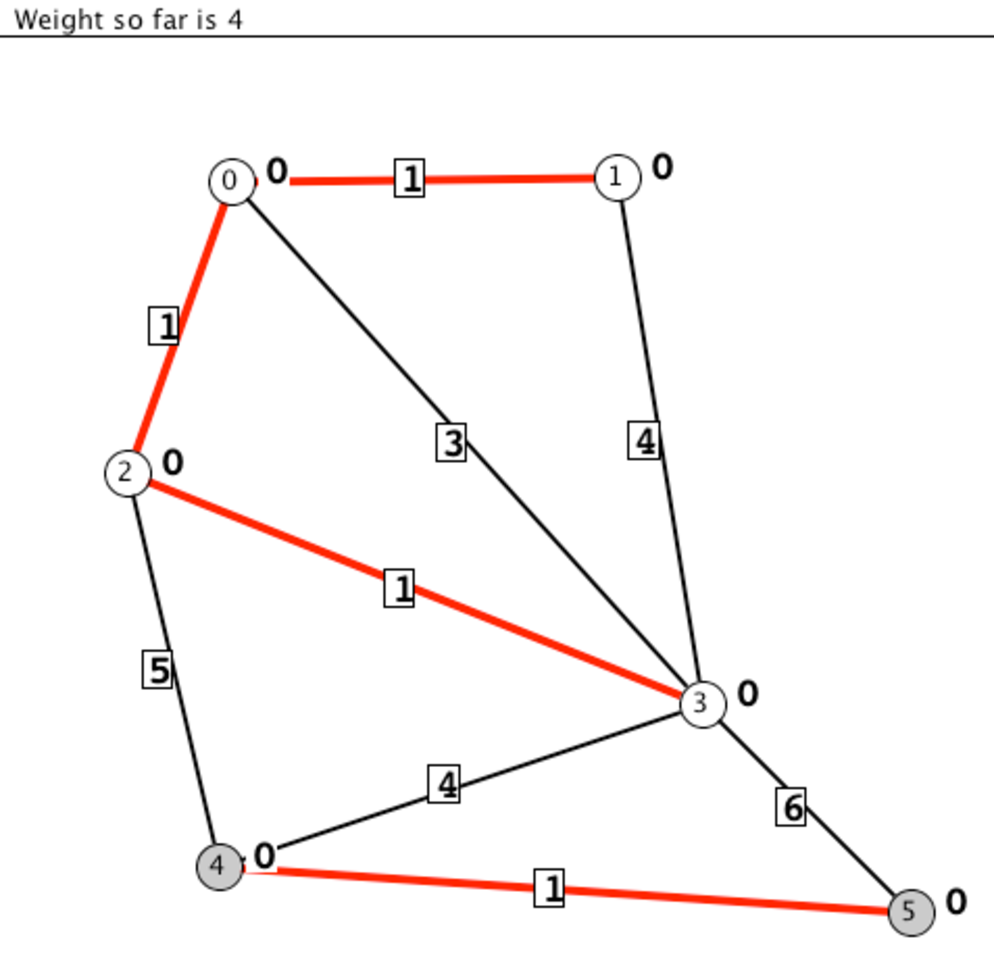
\includegraphics[scale=0.55]{X_kruskal_1}
}

(a) An edge is added to the tree.

\fbox{
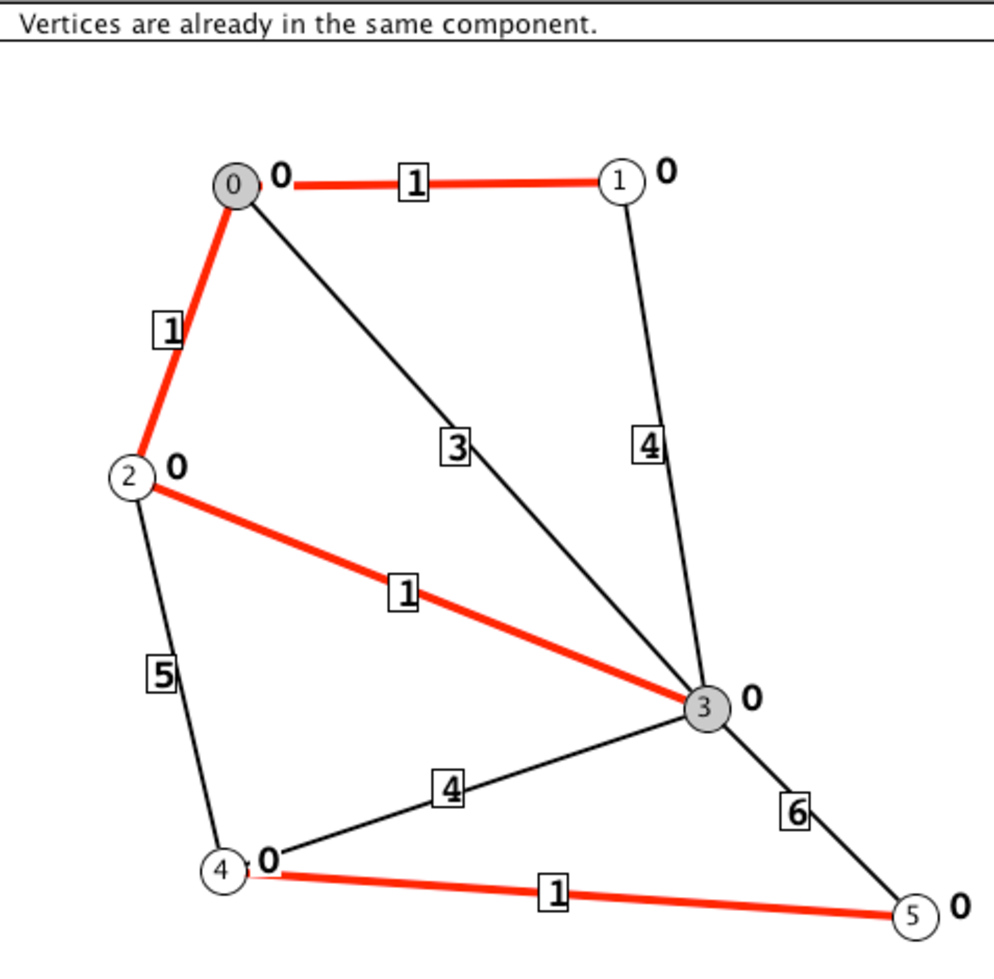
\includegraphics[scale=0.55]{X_kruskal_2}
}

(b) The current edge creates a cycle.

\end{center}

\caption{Two steps in Kruskal's algorithm. A message at the top left of the window describes the state of the algorithm.}

\label{fig:kruskal_pictures}
\end{figure}


Another simple algorithm implementation is that of Kruskal's algorithm
for finding a minimum spanning tree (or forest) in a graph.
Fig.~\ref{fig:kruskals_algorithm}
shows the implemented animation of Kruskal's algorithm.
Additional Galant features/workarounds illustrated here are:
\begin{itemize}

\item
Use of the keyword \verb+function+ to declare a function: this avoids the
syntactic complications of Java method declarations. In the case of
\verb+FIND_SET+, for example, you would normally have to say\\
\verb+static Node FIND_SET( Node x )+\\
and would get error messages about non-static methods in a static context
if you omitted the keyword \verb+static+.

\item
Implicit use of weights to sort the edges: weights are created by the
explorer when editing a graph. The only (syntactic) drawback is the required
use of the Java \verb+Collections.sort()+ construct, but this will be easy to fix in future releases.
Another piece of awkward syntax is the template invocation
\verb+List<Edge>+; again, this is easily fixable.

\item
The ability to write messages during execution, as accomplished by the
\verb+writeMessage+ calls.
The syntax that requires \verb+writeMessage+ to be a method of the \verb+Graph+
class is awkward, but can be remedied by augmenting the macro translation
mechanism.

\item
Declaration of a global array: the current implementation of Galant does
not provide a less Java-specific variant.
With moderate effort the Galant preprocessor could be augmented to provide
a more transparent syntax, such as\\
\verb+Node array parent[Node]+\\
The underlying implementation could either be a map (associative array) or an
array with integer indices but with nodes automatically converted to their
id's so that a reference to an element would always be \verb+parent[x]+
rather than \verb+parent[x.getId()]+.
In this specific situation -- implementation of disjoint set union --
the need for the array can be obviated by providing disjoint sets as
a built-in data structure.

\end{itemize}

Two steps in the execution of the animation are shown
in Fig.~\ref{fig:kruskal_pictures}.
The two endpoints of an edge are marked when that edge is considered
for inclusion in the spanning tree.
If the endpoints are not in the same tree, the edge is added and highlighted
and the cost of the current tree is displayed in the message.
Otherwise the message reports that the endpoints are already in the same tree. 
